\section{Mathematical Framework}
\label{sec:mathematical_framework}

This section extends the second-order cone model of the harmonic hosting capacity problem for phase-balanced three-phase power systems presented in~\cite{} to an robust optimization problem, hedging against four distinct sources of uncertainty:
\begin{enumerate}
    \item [\S\ref{sec:reference_bus_harmonic_voltage})] reference bus harmonic voltage,
    \item [\S\ref{sec:bus_fundamental_voltage})] bus fundamental voltage,
    \item [\S\ref{sec:bus_shunt_impedance})] bus shunt impedance, and
    \item [\S\ref{sec:edge_impedance})] edge impedance. 
\end{enumerate}

To this end, only the original constraints affected by the aforementioned uncertainties are highlighted and their robust counterparts are presented. The full model is presented in Appendix~\ref{sec:optimization_model}.


short explenation on min\_box approach
\begin{IEEEeqnarray}{0 l}
    \leq \min_{x\in [-1,1]^{n}} c^{T} x  \\
    \min(c,-c) \\
    = -\max(-c,c) = -|c| 
\end{IEEEeqnarray}

TODO (BL) : Swapping min_L,C always give upper bound because of min-max thm. Explain that is also exact for individual harmonic

\newpage

\subsection{Reference Bus Harmonic Voltage}
\label{sec:reference_bus_harmonic_voltage}

\noindent
Purpose: evaluate the impact of background harmonic distortion.

\noindent
Uncertain Parameters:~$\RealRefVoltage_{\Node,\Harmonic},~\ImaginaryRefVoltage_{\Node,\Harmonic}~\forall \Node \in \RefNodeSet, \Harmonic \in \HarmonicSet$

\noindent
Constraints:
\begin{IEEEeqnarray}{ 0 l }
    \text{reference bus voltage --~} \forall \Node \in \RefNodeSet, \Harmonic \in \HarmonicSet: \nonumber\\
    \quad \RealVoltage_{\Node,\Harmonic} = \RealRefVoltage_{\Node,\Harmonic}, \label{eq_ref_bus_volt_source_a} \\ 
    \quad \ImaginaryVoltage_{\Node,\Harmonic} = \ImaginaryRefVoltage_{\Node,\Harmonic}, \label{eq_ref_bus_volt_source_b}
\end{IEEEeqnarray}

\noindent
Perturbation Set: 
\begin{IEEEeqnarray}{ 0 r C l }
    \mathcal{Z} = \{ \zeta \in \mathbb{R}^{L}: \exists u \in \mathbb{R}^{K}: P\zeta + Qu + p \in \bold{K}\} (?).
\end{IEEEeqnarray}

A robust approach hedges against the worst-case realisation of the uncertainty, the worst-case realisation of the uncertainty will always occur on the edge of the circle.

\begin{figure}[b!]
    \centering
    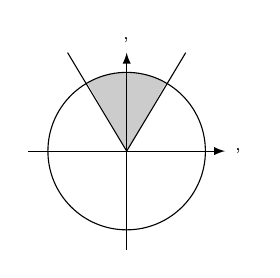
\begin{tikzpicture}
        % fill
        \fill[gray!40] (0.0,0.0) -- (-0.5,0.86603) --(-0.48481,0.87462) --(-0.46947,0.88295) --(-0.45399,0.89101) --(-0.43837,0.89879) --(-0.42262,0.90631) --(-0.40674,0.91355) --(-0.39073,0.9205) --(-0.37461,0.92718) --(-0.35837,0.93358) --(-0.34202,0.93969) --(-0.32557,0.94552) --(-0.30902,0.95106) --(-0.29237,0.9563) --(-0.27564,0.96126) --(-0.25882,0.96593) --(-0.24192,0.9703) --(-0.22495,0.97437) --(-0.20791,0.97815) --(-0.19081,0.98163) --(-0.17365,0.98481) --(-0.15643,0.98769) --(-0.13917,0.99027) --(-0.12187,0.99255) --(-0.10453,0.99452) --(-0.08716,0.99619) --(-0.06976,0.99756) --(-0.05234,0.99863) --(-0.0349,0.99939) --(-0.01745,0.99985) --(0.0,1.0) --(0.01745,0.99985) --(0.0349,0.99939) --(0.05234,0.99863) --(0.06976,0.99756) --(0.08716,0.99619) --(0.10453,0.99452) --(0.12187,0.99255) --(0.13917,0.99027) --(0.15643,0.98769) --(0.17365,0.98481) --(0.19081,0.98163) --(0.20791,0.97815) --(0.22495,0.97437) --(0.24192,0.9703) --(0.25882,0.96593) --(0.27564,0.96126) --(0.29237,0.9563) --(0.30902,0.95106) --(0.32557,0.94552) --(0.34202,0.93969) --(0.35837,0.93358) --(0.37461,0.92718) --(0.39073,0.9205) --(0.40674,0.91355) --(0.42262,0.90631) --(0.43837,0.89879) --(0.45399,0.89101) --(0.46947,0.88295) --(0.48481,0.87462) --(0.5,0.86603) -- cycle;
        % axis
        \draw [-latex] (-1.25,0.00) -- (1.25,0.0) node [right] {\footnotesize $\ImaginaryRefVoltage_{\Node,\Harmonic}$};
        \draw [-latex] (0.00,-1.25) -- (0.00,1.25) node [above] {\footnotesize $\RealRefVoltage_{\Node,\Harmonic}$};
        % p = 2
        \draw (0.00,0.00) circle (1.00);
        \draw (0.00,0.00) -- (-0.75,1.25);
        \draw (0.00,0.00) -- ( 0.75,1.25);
    \end{tikzpicture}
    \caption{Illustration of uncertainty set of the reference bus harmonic voltage.}
    \label{fig:reference bus harmonic voltage}
\end{figure}

\newpage

\subsection{Bus Fundamental Voltage}
\label{sec:bus_fundamental_voltage}

\noindent
Purpose: evaluate the impact of power system operation, i.e, fundamental voltage magnitude.

\noindent
Uncertain Parameters:~$\FundamentalVoltageMagnitude{\Node},~\forall \Node \in \NodeSet$

\noindent
Constraints:
\begin{IEEEeqnarray}{ 0 l } 
    \text{root mean square voltage --~} \forall \Node \in \NodeSet: \nonumber \\
    \quad \sum_{\Harmonic \in \HarmonicSet} (\RealVoltage_{\Node,\Harmonic})^{2} + (\ImaginaryVoltage_{\Node,\Harmonic})^{2} \leq (\MaximumVoltage_{\Node})^{2} - (\FundamentalVoltageMagnitude{\Node})^{2}, \label{eq:soc_rms} \\
    \text{total harmonic voltage --~} \forall \Node \in \NodeSet: \nonumber \\
    \quad \sum_{\Harmonic \in \HarmonicSet} (\RealVoltage_{\Node,\Harmonic})^{2} + (\ImaginaryVoltage_{\Node,\Harmonic})^{2} \leq (\textit{THD}_{\Node}^{\text{u}})^2\,(\FundamentalVoltageMagnitude{\Node})^{2},  \label{eq:soc_thd} \\
    \text{individual harmonic voltage --~} \forall \Node \in \NodeSet, \Harmonic \in \HarmonicSet: \nonumber \\
    \quad (\RealVoltage_{\Node,\Harmonic})^{2} + (\ImaginaryVoltage_{\Node,\Harmonic})^{2} \leq (\textit{IHD}^{\text{u}}_{\Node,\Harmonic}\,\FundamentalVoltageMagnitude{\Node})^{2},
    \label{eq:soc_ihd}
\end{IEEEeqnarray}

\noindent
Perturbation Set:
\begin{IEEEeqnarray}{ 0 r C l }
    \mathcal{Z} = \text{Box}_{1} \equiv \{ \zeta \in \mathbb{R}:~\|\zeta\|_{\infty} \leq 1 \}.
\end{IEEEeqnarray}

Even better would be to split this up into two random parameter, one global fundamental voltage parameter~$\VoltageParameter^{\text{mag,fund,global}}$ and a local fundamental voltage parameter~$\VoltageParameter^{\text{mag,fund,local}}_{\Node}$, such that:
\begin{IEEEeqnarray}{ 0 r C l }
    \FundamentalVoltageMagnitude{\Node} &=& \VoltageParameter^{\text{mag,fund,global}} + \VoltageParameter^{\text{mag,fund,local}}_{\Node}
\end{IEEEeqnarray}
Both random parameters would have a perturbation set as illustrated in Fig.~\ref{fig:bus_fundamental_voltage}.

\begin{figure}[b!]
    \centering
    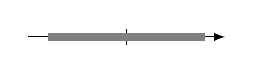
\begin{tikzpicture}
        % axis
        \draw (0.00,-0.10) -- (0.00,0.10);
        \draw [-latex] (-1.25,0.00) -- (1.25,0.0) node [right] {\footnotesize $\FundamentalVoltageMagnitude{\Node}$};
        % p = inf
        % \draw (0.00,0.00) circle (1.00);
        \draw [gray, line width=1mm] (-1.00,0.00) -- (1.00,0.00);
        % \draw (0.00,0.00) -- ( 0.75,1.25);
    \end{tikzpicture}
    \caption{Illustration of uncertainty set of the bus fundamental voltage.}
    \label{fig:bus_fundamental_voltage}
\end{figure}

\newpage

\subsection{Bus Shunt Impedance}
\label{sec:bus_shunt_impedance}

\noindent
Purpose: Evaluate the impact of shunt compensation and (a)synchronous motor load parameter uncertainty.

\noindent:
Uncertainty sources: power of connected load, $\cos(\varphi)$, start vs nominal current-ratio, RX-ratio, etc.

\noindent
Uncertain Parameters:~$\ShuntConductance{\Node,\Harmonic},~\ShuntSusceptance{\Node,\Harmonic},~\forall \Node \in \NodeSet, \Harmonic \in \HarmonicSet$

\noindent
Constraints:
\begin{IEEEeqnarray}{ 0 l }
    \text{Kirchhoff's current law --~} \forall \Node \in \NodeSet, \Harmonic \in \HarmonicSet: \nonumber \\
    \quad \sum_{\Edge\Node\AltNode \in \EdgeTupleSet} \mkern-6mu \RealCurrent_{\Edge\Node\AltNode,\Harmonic} + \mkern-9mu
    \sum_{\UnitTuple \in \UnitTupleSet} \mkern-6mu \RealCurrent_{\UnitTuple,\Harmonic}  + \ShuntConductance{\Node,\Harmonic} \RealVoltage_{\Node,\Harmonic} -\ShuntSusceptance{\Node,\Harmonic} \ImaginaryVoltage_{\Node,\Harmonic}  = 0, \label{eq:kcl_node_real} \\
    \quad \sum_{\Edge\Node\AltNode \in \EdgeTupleSet} \mkern-6mu \ImaginaryCurrent_{\Edge\Node\AltNode,\Harmonic} + \mkern-9mu
    \sum_{\UnitTuple \in \UnitTupleSet} \mkern-6mu \ImaginaryCurrent_{\UnitTuple,\Harmonic} + \ShuntConductance{\Node,\Harmonic} \ImaginaryVoltage_{\Node,\Harmonic} + \ShuntSusceptance{\Node,\Harmonic} \RealVoltage_{\Node,\Harmonic}= 0, \label{eq:kcl_node_imag} \\
\end{IEEEeqnarray}

\noindent
Perturbation Set:
\begin{IEEEeqnarray}{ 0 r C l }
    \mathcal{Z} = \text{Box}_{1} \equiv \{ \zeta \in \mathbb{R}^{2}:~\|\zeta\|_{\infty} \leq 1 \}.
\end{IEEEeqnarray}

Even more accurate would be a rectangle shape rather than a square. 

\begin{figure}[b!]
    \centering
    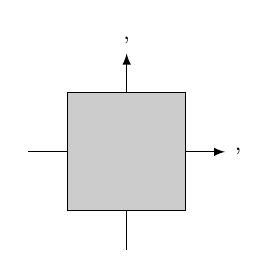
\begin{tikzpicture}
        % axis
        \draw [-latex] (-1.25,0.00) -- (1.25,0.0) node [right] {\footnotesize $\ShuntSusceptance{\Node,\Harmonic}$};
        \draw [-latex] (0.00,-1.25) -- (0.00,1.25) node [above] {\footnotesize $\ShuntConductance{\Node,\Harmonic}$};
        % p = inf
        \draw [fill=gray!40] (0.75,0.75) rectangle (-0.75,-0.75);
    \end{tikzpicture}
    \caption{Illustration of uncertainty set of the nodal shunt admittance.}
    \label{fig:nodal_shunt_admittance}
\end{figure}

\newpage

\subsection{Edge Impedance}
\label{sec:edge_impedance}

\noindent
Purpose: Evaluate the impact of cable, overhead-line and transformer parameter uncertainty. 

\noindent
Uncertainty sources: geometry and positioning of a cable, engineering data of a transformer.

\noindent
Uncertain Parameters:~$\SeriesResistance{\Line,\Harmonic},~\SeriesReactance{\Line,\Harmonic},~\ShuntConductance{\LineTuple,\Harmonic},~\ShuntSusceptance{\LineTuple,\Harmonic},~\forall \LineTuple \in \LineTupleSet, \Harmonic \in \HarmonicSet$

\noindent
Constraints:
\begin{IEEEeqnarray}{ 0 l } 
\text{Ohm's law --~} \forall \LineTuple \in \LineTupleSetFr, \Harmonic \in \HarmonicSet: \nonumber\\
    \quad \RealVoltage_{\AltNode,\Harmonic} = \RealVoltage_{\Node,\Harmonic} - 
    \SeriesResistance{\Line,\Harmonic} \RealSeriesCurrent_{\LineTuple,\Harmonic} +
    \SeriesReactance{\Line,\Harmonic} \ImaginarySeriesCurrent_{\LineTuple,\Harmonic}, \label{eq:ol_real} \\
    \quad \ImaginaryVoltage_{\AltNode,\Harmonic} = \ImaginaryVoltage_{\Node,\Harmonic} - 
    \SeriesResistance{\Line,\Harmonic} \ImaginarySeriesCurrent_{\LineTuple,\Harmonic} -
    \SeriesReactance{\Line,\Harmonic} \RealSeriesCurrent_{\LineTuple,\Harmonic}, \label{eq:ol_imag} \\
    \text{branch total current --~} \forall \LineTuple \in \LineTupleSet, \Harmonic \in \HarmonicSet: \nonumber \\
    \quad \RealCurrent_{\LineTuple,\Harmonic} =
    \ShuntConductance{\LineTuple,\Harmonic} \RealVoltage_{\Node,\Harmonic} - 
    \ShuntSusceptance{\LineTuple,\Harmonic} \ImaginaryVoltage_{\Node,\Harmonic} +
    \RealSeriesCurrent_{\LineTuple,\Harmonic}, \label{eq:btc_real} \\
    \quad \ImaginaryCurrent_{\LineTuple,\Harmonic} =
    \ShuntConductance{\LineTuple,\Harmonic} \ImaginaryVoltage_{\Node,\Harmonic} + 
    \ShuntSusceptance{\LineTuple,\Harmonic} \RealVoltage_{\Node,\Harmonic} +
    \ImaginarySeriesCurrent_{\LineTuple,\Harmonic}, \label{eq:btc_imag} 
\end{IEEEeqnarray}

\noindent
Perturbation Set:
\begin{IEEEeqnarray}{ 0 r C l }
    \mathcal{Z} = \text{Box}_{1} \equiv \{ \zeta \in \mathbb{R}^{4}:~\|\zeta\|_{\infty} \leq 1 \}.
\end{IEEEeqnarray}

\newpage

\subsection{Minimal Example}

Consider a single purely-inductive branch, i.e.,~$R=0$, with a generator setting a clean voltage at node one, i.e.,~$\bar{U}_{1}=0$, and a shunt capacitance at node two. In this minimal example, the maximum harmonic real unit current, i.e.,~$\mathfrak{I}(\bar{I}_{h}^{u})=0$ is determined that can be injected at node two for the third and fifth harmonic~$h$, considering independent box uncertainty on the inductance and capacitance, without the voltage at node two exceeding~$U^{max}$. 

As a consequence of the branch resistance being zero and the harmonic imaginary current being zero, the induced voltage at node two is purely imaginary, i.e.,~$\mathfrak{R}(\bar{U}_{2,h})=0$.

This results in a minimal example of three non-zero variables for each harmonic~, i.e.,~$\mathfrak{R}(\bar{I}^{u}_{h})$,~$\mathfrak{R}(\bar{I}^{g}_{h})$, and~$\mathfrak{I}(\bar{U}_{2,h})$, subsequently, for brevity, denoted as~$I^{u}_{h}$,~$I^{g}_{h}$, and~$U_{h}$, respectively.

\begin{figure}[ht!]
    \centering
    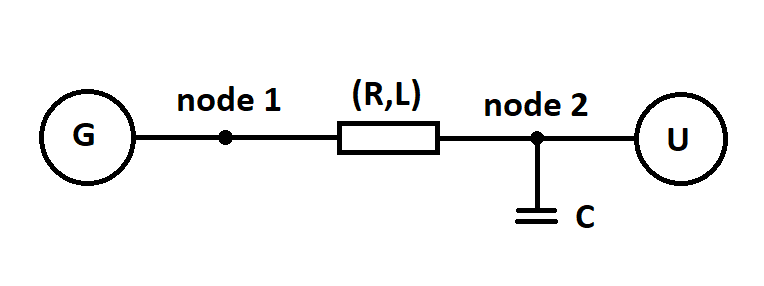
\includegraphics[width=0.5\linewidth]{figures/minimal_example_robust.png}
\end{figure}

Sets:\newline
$h \in \{3,5\}$

Deterministic parameters:\newline
$U^{max} = 0.01$\newline
$w=2 \pi f \approx 314.1592$

Robust parameters:\newline
$0.2\cdot10^{-3} \leq C \leq 0.4\cdot10^{-3}$\newline
$1.0\cdot10^{-3} \leq L \leq 2.0\cdot10^{-3}$,\newline
where~$L$ and~$C$ are independent

The problem is expressed as a robust linear problem in the form:~$\{\min~c^{T}x,~\text{s.t.}~Ax \leq b\}.$

Variables:\newline
$x = [I^{u}_{3},I^{u}_{5},I^{g}_{3},I^{g}_{3},U_{3},U_{5}]$\newline
$c = [-1,-1,0,0,0,0]$\newline
$A = \begin{bmatrix}
        -1      & 0     & 1     & 0     & 3wC   & 0     \\
        0       & -1    & 0     & 1     & 0     & 5wC   \\
        1       & 0     & -1    & 0     & -3wC  & 0     \\
        0       & 1     & 0     & -1    & 0     & -5wC  \\
        0       & 0     & 3wL   & 0     & 1     & 0     \\
        0       & 0     & 0     & 5wL   & 0     & 1     \\
        0       & 0     & -3wL  & 0     & -1    & 0     \\
        0       & 0     & 0     & -5wL  & 0     & -1    \\
        0       & 0     & 0     & 0     & -1    & 0     \\
        0       & 0     & 0     & 0     & 0     & -1    \\
        0       & 0     & 0     & 0     & 1     & 0     \\
        0       & 0     & 0     & 0     & 0     & 1     \\  
\end{bmatrix}$, \newline where lines 1-4 are reformulated equality constraints representing Kirchhoff's current law, lines 5-8 are reformulated equality constraints representing Ohm's law, and lines 9-12 are inequality constraints on the harmonic voltage at node two. 
$b = [0,0,0,0,0,0,0,0,0,0,U^{max},U^{max}]$

\newpage
~
\newpage